This report is structured as follows. After explaining the project requirements, three main equipments for the project is introduced. Section 2 follows with the explanation of the vision algorithm used to achieve the goal of the project. Our Drone flight-plans are elaborated in section 3 by comparing two possible plans our team came up with. Two types of simulation were conducted before the tournament, elaborated in Section 4 along with the result analysis. The competition result, as well as the discussion, follows in section 5. Section 6 finally wrap the report with few concluding remarks.

\subsection{Project assignment}
The goal of the project is to develop a flight plan for an AR Drone 2.0 to fly in the Cyber Zoo with a flight time of 10 minutes (equipment. Within this time, the drone should be avoiding obstacles in the fixed area purely based on the vision data from the front camera of the drone. Examples of the obstacles with one obvious color are given but the vision algorithm should detect an obstacle based on more possible obstacle colors. The program should be set beforehand and during the flight no human intervention is allowed, so the drone should know when

\subsection{AR Drone: A Quad-rotor MAV}
A Quad-rotor named AR Drone 2.0 is the chosen MAV in this project. The first version of the vehicle was build by the Parrot company (France) in 2004, and released for public in 2010, aiming for the market of video games and home entertainment\cite{Bristeau:11}. The platform of the vehicle is a Quad-rotor, a four fixed propeller that are rotated by four brushless motors, each controlled by an ATMEGA8L 8bit microcontroller. The AR.Drone is equipped with 3 cells battery that supplies 11.1 V and 1000 mAh providing power for 10 to 15 minutes of flight. The platform is very popular in MAV research field\cite{Bristeau:11}\cite{Pestana:13}\cite{Lugo:14}, since it has the capability of both hovering and fast forward cruising. In order to make the vehicle acceptable for public, a very effective control and stabilization system is mandatory for a easy piloting platform. The general view of the AR Drone 2.0, the one used for this project, is shown in Figure~\ref{f:TheDrone} below.

\begin{figure}
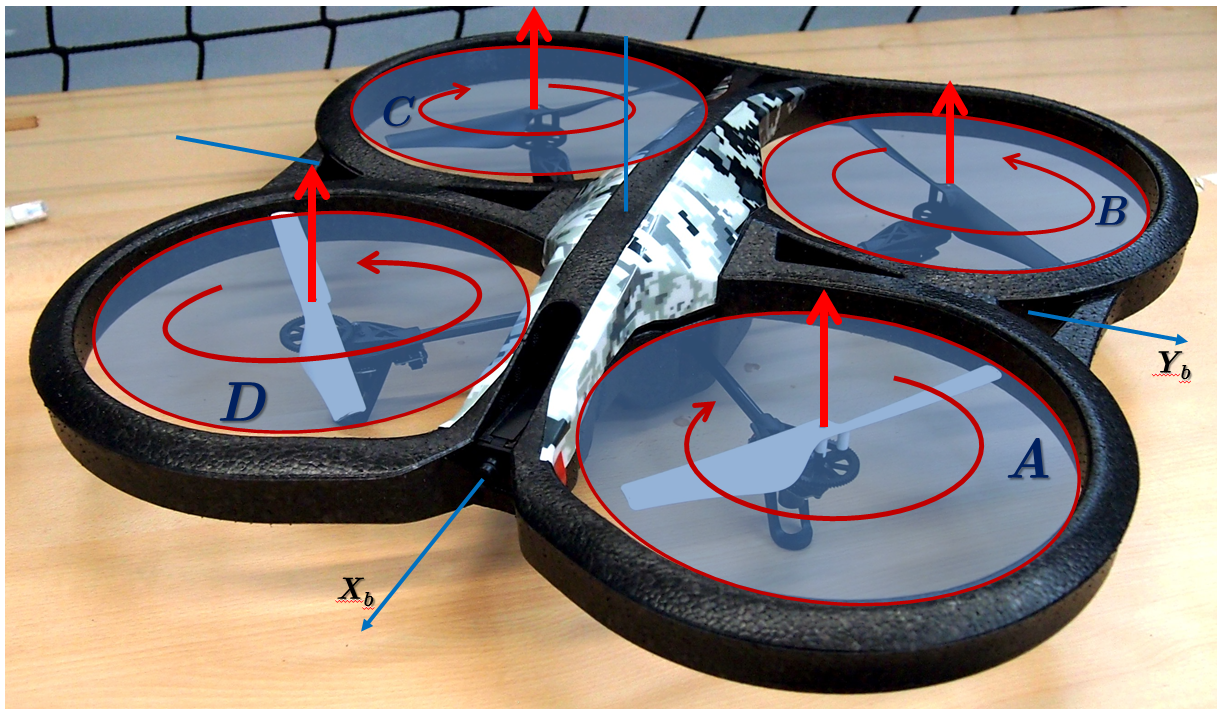
\includegraphics[width=1\linewidth]{Figures/TheDrone.png}
\centering
\caption{The AR Drone 2.0 from the Parrot Inc (France) - with schematic of the four propellers direction of rotation}
\label{f:TheDrone}
\end{figure}

Quad-rotor is controlled by adjusting the thrust and rotation combination of its propellers. AR Drone propeller setup is as shown in Figure~\ref{f:TheDrone}, where two of the propeller (A and C) turn clockwise, while the other two (B and D) turn counter clockwise. On stationary hover condition, every propeller produce the same thrust from the same RPM. Torque from each motor, therefore, are canceled by the combination of propeller rotation. To have a positive pitching motion, more power is given to propeller B and C, while reducing power in A and D to keep the balance with the weight and the desired forward/backward speed. Rolling motion is controlled in similar manner, positive rolling is achieved by giving more power to A and B, while reducing power in C and D. Finally, positive yawing is controlled by giving more power to propeller A and C, while reducing power in B and D. Controlling task for stability is challenging, because the rotational motion, i.e, roll, pitch and yaw, and the translational motions, i.e., heave, sway, and surge, are coupled. The work of \cite{Bouabdallah:07} elaborated this challenge comprehensively.

The Guidance, Navigation, and Control system of AR.Drone is supported by an a set of sensory system consisting a 3-axis accelerometer, a 2-axis gyroscope, a 1-axis gyroscope, and two ultrasonic sensors. The ultrasonic sensor is used for altitude and vertical displacement estimation, while the other is part of an Inertial Measurement Unit (IMU) that is essential for control and stability of the vehicle.All the sensors is chosen to be as low-cost as possible, which implies that the embedded control system have to deal with a lot of bias, misalignment angles, and other errors\cite{Bristeau:11}. Furthermore, two cameras are equipped in AR.Drone, which are not mainly intended to be used as sensor for the flight. Coupled with the IMU rotation measurement and vision algorithms (explained in the next section), however, the camera can be used in vertical speed estimation (camera pointed down). 

\subsection{CyberZoo and OptiTrack}
At march the 5th, 2014, TU Delft's so called \textbf{Cyber Zoo} is opened as a new research and test laboratory for robots and unmanned vehicles. Initiated by the TU Delft Robotic Institute, this facility is a 10 x 10 meters area covered by 7 meter high net. The facility is located in the hangar of the Faculty of Aerospace Engineering, and it is the designated field in which the project MAV will be flown.

The Cyberzoo is equipped with a three dimensional optical motion tracking system based on called OptiTrack by NaturalPoint Inc\cite{Hansen:14}\cite{Guadarrama-Olvera:14}. The system consist of 24 camera, observed in Figure~\ref{f:OptiTrackCyberZoo},  to triangulate the position of retro-reflective markers, placed on the surface of a motion platform in a specific distance between each other, such as shown in Figure~\ref{f:Markers} below. By defining a set of marker positions as a rigid body, the OptiTrack system can recognized the particular pattern and track the motion continuously in a screen, also shown in Figure~\ref{f:OptiTrackCyberZoo}. The OptiTrack then provide, through a UDP connection, a local positioning data that is almost similar with the data provided by a GPS. with the This OptiTrack system is known to be a low-cost system that have accuracy comparable with its more high end competition, the well established Vicon motion capture system\cite{Hansen:14}.

\begin{figure}[h]
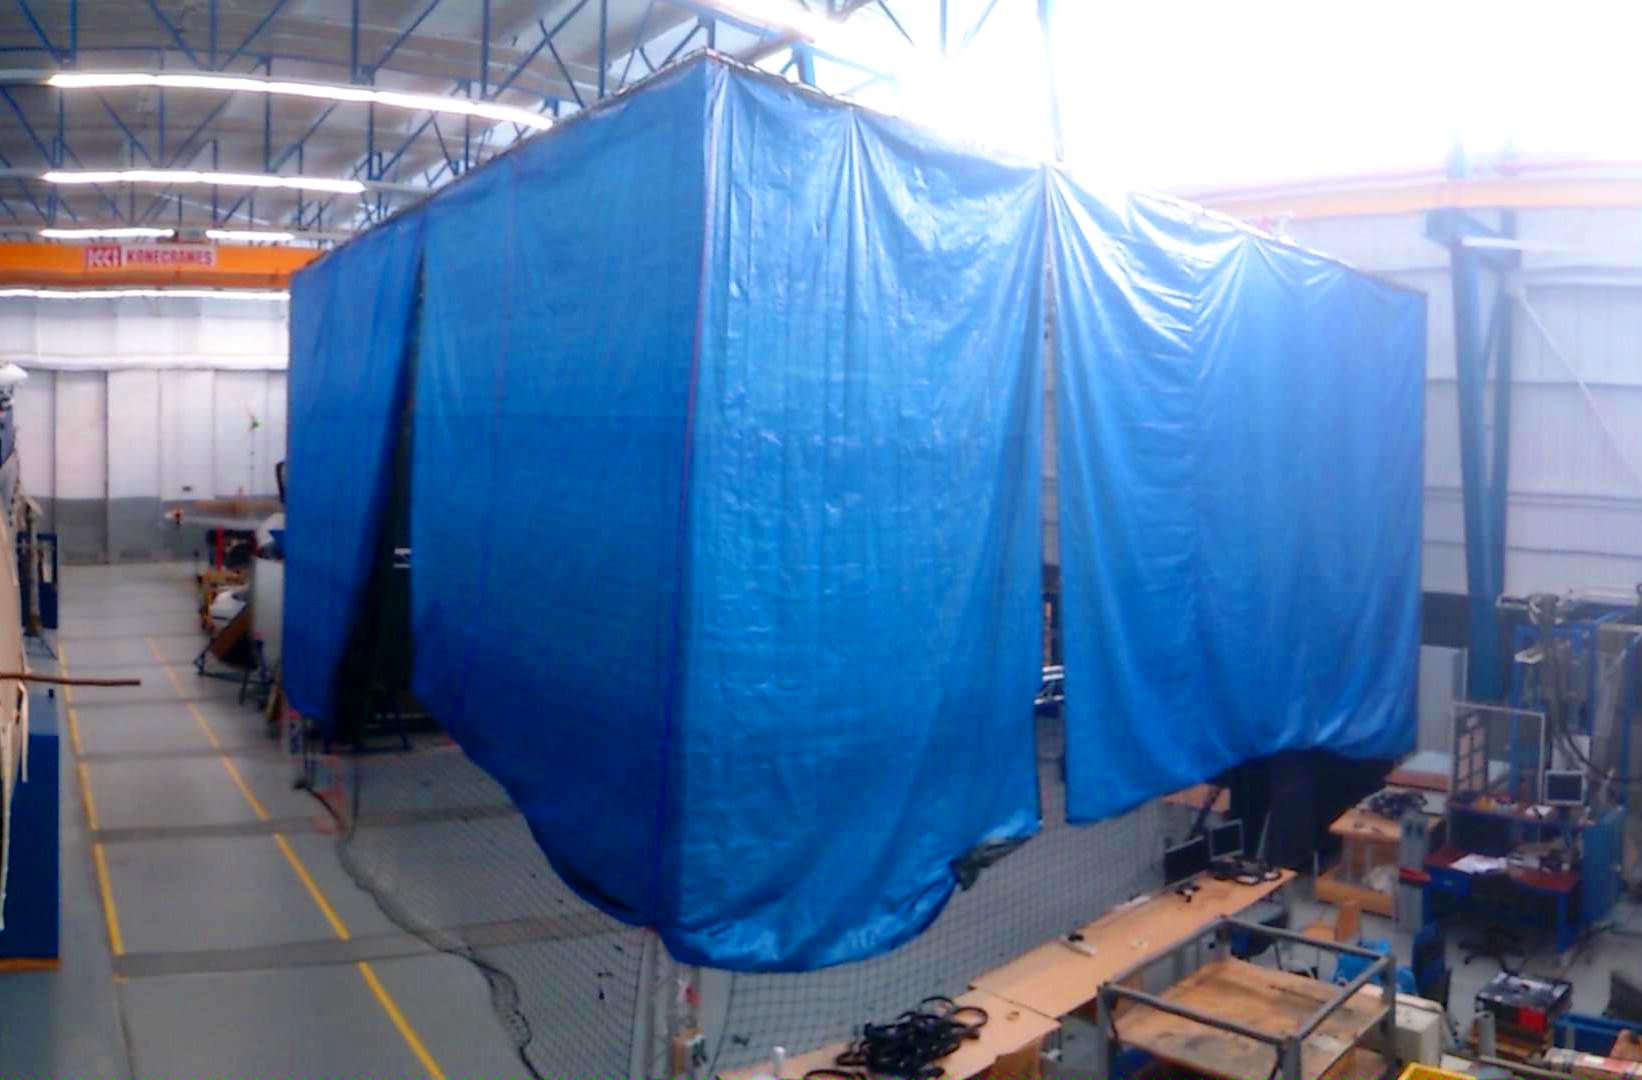
\includegraphics[width=0.9\linewidth]{Figures/TheCyberZoo.png}
\centering
\caption{The cyber zoo inside the hangar of the Faculty of Aerospace Engineering, Delft University of technology. Currently covered by a thick canvas that serves as a background for computer vision for the robots inside}
\label{f:TheCyberZoo}
\end{figure}

\begin{figure}[h]
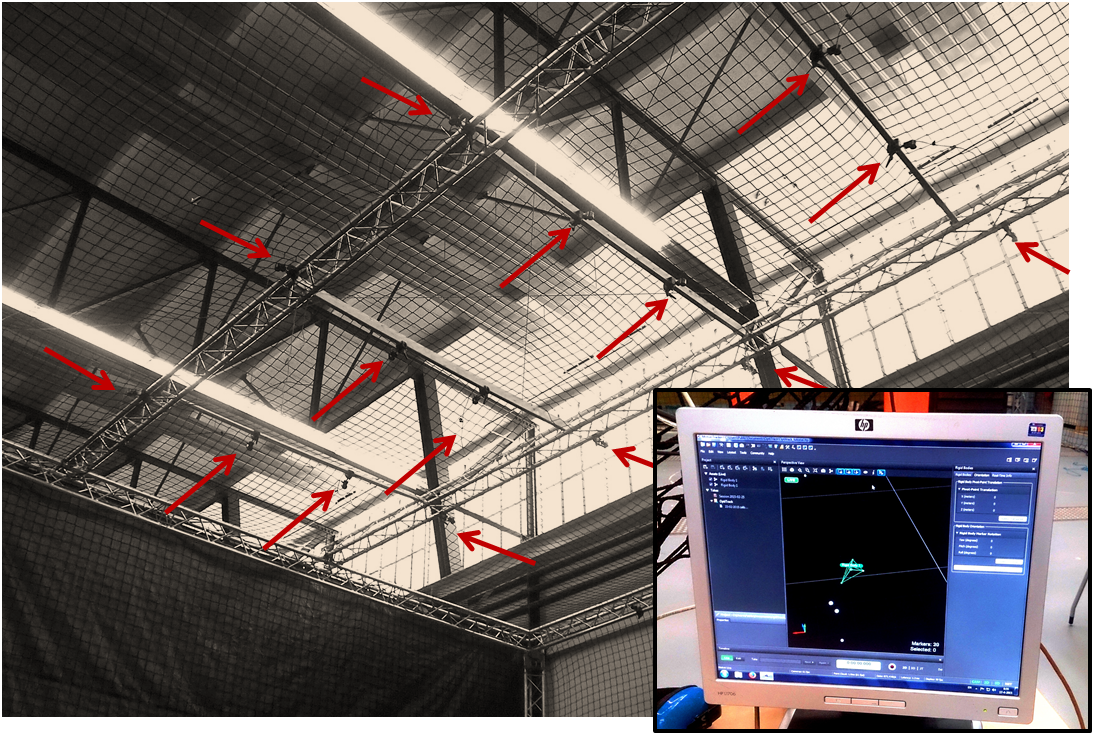
\includegraphics[width=0.9\linewidth]{Figures/OptiTrackCyberZoo.png}
\centering
\caption{Some camera positions on the roof of the cyber zoo. (inset) the OptiTrack GUI that combines data from the 24 camera to triangulate marker positions inside the cyberzoo}
\label{f:OptiTrackCyberZoo}
\end{figure}

\begin{figure}[h]
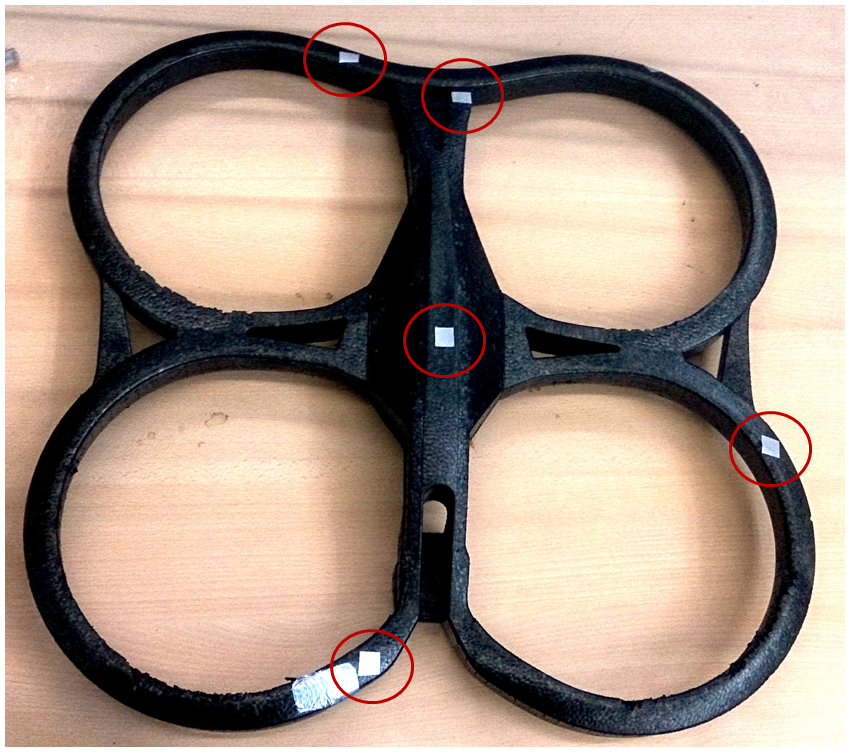
\includegraphics[width=0.7\linewidth]{Figures/Markers.png}
\centering
\caption{Retro-reflective marker is installed on the surface of AR.Drone hull. Each Hull have a specific position combination that can be recorded and tracked by the OptiTrack system}
\label{f:Markers}
\end{figure}

\subsection{Paparazzi: Open Source Autopilot}
The AR.Drone in this project will be equipped with the open source autopilot system Paparazzi, which is mainly developed and maintained by the Ecole Nationale de l'Aviation Civile (ENAC) in Toulousse, France. The system run in a Linux platform, and has been used by hundreds of research from all around the world\cite{Reuder:12}\cite{Royo:11}. The opening window of this software is shown in the Figure below.

%Figure Paparazzi

Paparazzi's Ground Control Station (GCS) is used to determined the flight plan of a vehicle to fly autonomously. The flight plan is mainly set using combination of several blocks, or modules, embedded in the GCS, e.g., the take-off, set direction to a waypoint, go to a waypoint, or go make a circle. A wifi connection is established between Paparazzi and the vehicle for a two-way communications, enabling the AR Drone to sent its states back to the GCS and operator. The flight plans can be interrupted by the operator anytime during the flight.

Inside the cyber zoo, however, the states of position is not given directly by the drone, since it is flying in a GPS-denied environment. Instead, Paparazzi must be modified to receive data from the OptiTrack local positioning. This is done by using the NavNet module in Paparazzi, coupled with a view changes in the airframe and flight plan code. The local position data from each rigid body is sent through a UDP connection, and therefore the computer platform, running Paparazzi in the CyberZoo, is required to have two connection port. 

